Wolfenstein 3D was released on May, 5th 1992 and established the First Person Shooter genre. The beautiful graphics, speed, high framerate, crisp sounds effects and engaging musics were universally acclaimed. Within a year more than 100,000 units had been sold over the mail\footnote{The game was distributed via shareware: You had to mail money to get the full version}, bringing fame and a little bit of fortune to the team who built it: id Software.\\
\\
The many fans did not stop at beating the game. Because they wanted to modify it and make their own characters and maps, they started to explore and reverse engineer the engine. Within a few months the assets formats were well known and people released mods\footnote{MODified version.} with altered graphics, sounds effects, music and maps. The core of the game however, the 3D engine and the secrets of its speed remained mostly unknown.\\
\\
It was kept secret for an obvious reason: A good game engine was considered the main asset of a game company. As a mean to outperform competitors it was a good business practice to keep other programmers  uneducated in order to gain technological advantage and generate profit.\\
\\
But a few people within id Software did not see things that way. Instead of going along with what was common sense, they wanted to embrace players enthusiasm and fully open the source code to the public. After many internal debate, id Software did the unthinkable: On July 21, 1995 they uploaded a zip archive on \emph{ftp.idsoftware.com} containing the full source code of the engine with all instructions to build it\footnote{They were not totally crazy: They had built a game engine making Wolfenstein 3D obsolete: Doom was released on December 10, 1993}.\\

 \begin{fancyquotes}
   Programming is not a zero-sum game. Teaching something to a fellow programmer doesn't take it away from you. I'm happy to share what I can, because I'm in it for the love of programming.\\
   \\
\textbf{John Carmack - Programmer}
 \end{fancyquotes}\\
\\
Opening the code did not only allow MODding and educate programers. It had two unforeseen consequences:\\
\\
First, it allowed the software to live long after the target hardware and operating system died. With access to the source, programmers were able to maintain and port the engine to new hardware and operating systems: Twenty years after the release of Wolfenstein 3D you can still play the game on anything with a CPU, some RAM and a framebuffer. \\
\\
Second, it create a window back in time looking right into 1992. After having reviewed Quake III and Doom III on \emph{fabiensanglard.net} I thought i would have merely skimmed over Wolfenstein 3D engine and its "simple" raycasting technology. But when out of curiosity I took a deeper look, something stroke me and I could not stop. The more I read, the more I came to realize one very important thing: The target machine, the IBM PC, was designed for office work, not gaming. It was meant to crunch integers and display static screens for word processors and spreadsheets application. It is when I realized this fact that thought I may have a story to tell. What id Software\footnote{A few other companies, such as Origins and LucasArts where also doing amazing things: I focus on Id because we have the source code!} did in 1991 was not just program a machine: They re-purposed something built to do office work and turned it into the best gaming platform in the world.\\
\\
But why go through so much trouble? After all if you were a game company and you wanted to make video games, you had hardware dedicated to this very specific thing: video game console! The Megadrive, the NES and the Neo-Geo had sprite engine which albeit small limitations such as size and number allowed to move something on the screen by simply updating its $(x,y)$ coordinates. They were able to easy generate smooth animation at 60Hz. Heck if really you wanted to use a personal computer for gaming why not use an Amiga which was packed with coprocessors designed for animation?\\
\\
The reason seats within one word: Framebuffer. The kind of game they wanted to do could not be done with a sprite engine or tricks from a Copper\footnote{Nickname of a powerful Amiga co-processor allowing operations at vsync level}. They wanted to shake the gaming world by providing an immersive experience: In three dimensions. And in order to do that, every frames, 70 times per seconds, they wanted to draw a full screen, pixel per pixel, in a framebuffer and sent it to the screen. \\
\par
That task also required a particularly powerful CPU. No console or Amiga\footnote{Jimmy Maher advances an interesting theory in his book "The Future was here: The Commodore Amiga": People wanted to play First Person Shooter, which the Amiga architecture did not allow: This inability ultimately provoked the downfall of Commodore's best seller.} could do the job as the mips\footnote{Million Instructions Per Second.} graph shows.
\par
\begin{figure}[H]
\centering
  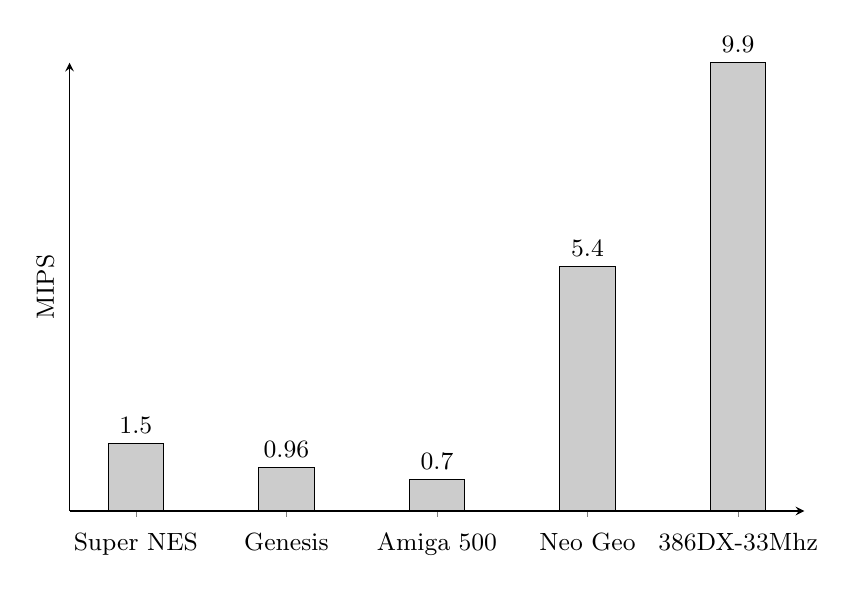
\begin{tikzpicture}[font=\small]
    \begin{axis}[
      width=0.9\textwidth,
      height=0.6\textwidth,
      ybar=6pt,
      bar width=20pt,
      ylabel={MIPS},
      ymin=0,
      ytick=\empty,
      xtick=data,
      axis x line=bottom,
      axis y line=left,
      enlarge x limits=0.11,
      symbolic x coords={Super NES,Genesis,Amiga 500,Neo Geo,386DX-33Mhz},
      xticklabel style={anchor=base,yshift=-\baselineskip},
      nodes near coords={\pgfmathprintnumber\pgfplotspointmeta}
    ]
      \addplot[fill=black!20,draw=black] coordinates {
        (Super NES,1.5)
        (Genesis,0.96)
        (Amiga 500,0.7)
        (Neo Geo,5.4)
        (386DX-33Mhz,9.9)
      };
    \end{axis}
   \end{tikzpicture}
   \caption{Game Console Vs PC: Raw power of the CPUs.} \label{fig:game_console_vs_PC}
 \end{figure}
 
So the IBM PC with its fast CPU and 256K framebuffer looked promising except there was two seemingly impossible to overcome obstacles:\\
\begin{itemize}
\item The video system (called VGA) had no double buffer. On paper it was not possible to have smooth animations.
\item The CPU could only do integer operations yet 3D engines and they trigonometric operations requires fractions.
\end{itemize}
And a myriad of mere difficulties:\\
\begin{itemize}
\item The RAM addressing mode was not flat but segmented resulting in complex and error prone pointer mathematics.
\item The pixel of the VGA were not square: the framebuffer was distorted when rendered on the screen.
\item The sound ecosystem was fragmented: Various sound systems had different capabilities and expectations.
\item The machine could only address 1MB or RAM. To go past that you had to enter a fragmented system of drivers called EMS and XMS.
\end{itemize}

At first sight it looked like the machine was DOOMed. Yet they made it happen and to help the readers understand the extend of the task, this book emphasis first on the hardware limitations then goes on to describe how the software circumvented and sometimes exploited these limitations:
\begin{itemize}
\item Chapter I: Hardware and its limits.
\item Chapter II: Team\footnote{This is an engineering book: The description is logistic. For the human aspect read David Kushner's chef d'oeuvre: "Masters of Doom''} pushing the edges.
\item Chapter III: Software, the Wolfenstein 3D game engine.
\end{itemize}
\par
\bu{Trivia :} The game was inspired by the 1981 Apple II title "Castle Wolfesntein" by Silas Warner. The Apple version was stealth oriented (Wolfesntein "Profound Carnage" 3D was a clear departure from the original theme) but really stood out thanks to its unprecedented use of digitized voices. Initially the team believed that they would be unable to use the Wolfenstein name due to trademark issues, and came up with multiple possible titles, only to discover that the original developer, Muse Software, had gone out of business several years earlier and let the trademark lapse, leaving them the option to name their game Wolfenstein 3D.

 \begin{figure}[H]
\centering
      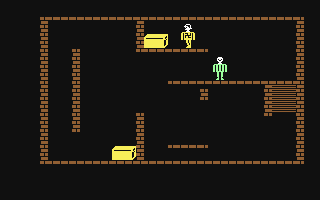
\includegraphics[width=\textwidth]{imgs/CastleWolfensteinC64.png}
\end{figure}

\note{Talk about Catacomb 3D and Hover Tank: As how much code was re-used for wolf3D.}
